\documentclass[../main.tex]{subfiles}
\graphicspath{{\subfix{..}}}

\begin{document}
\chapter{Neutrino physics}
\label{sec:neutrino}

\epigraph{I have done a terrible thing, I have postulated a particle that cannot be detected.}{Wolfgang Pauli -- ``Foreword'' by Frederick Reines to ``Spaceship Neutrino'' by Christine Sutton, (p. xi), 1992. }

%\textit{In chapter 1, I'll remind briefly the SM, its limitations, and give a short introduction to neutrino physics, with a reminder of the present important questions and a state of the art.}


\minitoc

Our understanding of the universe describes it as composed of elementary components called elementary particles; the study of these particles is therefore particle physics. The best established theoretical model describing these particles and their interactions is the Standard Model (SM).
The SM has successfully described many phenomena observed in particle physics over the past decades. However, a certain number of limitations affect the SM and suggest it is the manifestation at presently accessible energies of a more fundamental physics, which we call Physics Beyond the SM (BSM).

In this chapter, I describe briefly the Standard Model and its limitations in Section \ref{sec:neutrinos:sm}, then delve a bit further into the specifics of neutrino physics in Section \ref{sec:neutrino:th}.

\section{Introduction to the Standard model}
\label{sec:neutrinos:sm}

The SM categorizes elementary particles into two categories: the \textit{fermions} constituting matter and the \textit{bosons} that mediate their interactions. The fermions are themselves divided into two categories, the \textit{quarks} and the \textit{leptons}. Figure \ref{fig:neutrino:sm} shows the elementary particles and their classification. Each one of these particles is characterized by the value of their quantum numbers, the main ones being their mass $m$, spin $J$, electric charge $Q$, and the quantum numbers playing an analogue role for the weak (weak isospin) and strong interactions (color). The leptons also possess a lepton quantum number $L = 1$ and a flavor quantum number $L_{e,\mu,\tau}$ corresponding to their family: electron, muon, or tau. The leptons are thus split into three families: the electron $L_e = 1 \rightarrow (e, \nu_e)$, muon $L_\mu = 1 \rightarrow (\mu, \nu_\mu)$, and tau $L_\tau = 1 \rightarrow (\tau, \nu_\tau)$ families, each composed of a charged particle $Q = 1$ and a neutral particle $Q = 0$. The neutral leptons are named the \textit{neutrinos}, represented by the character $\nu$.

\begin{figure}
  \centering
  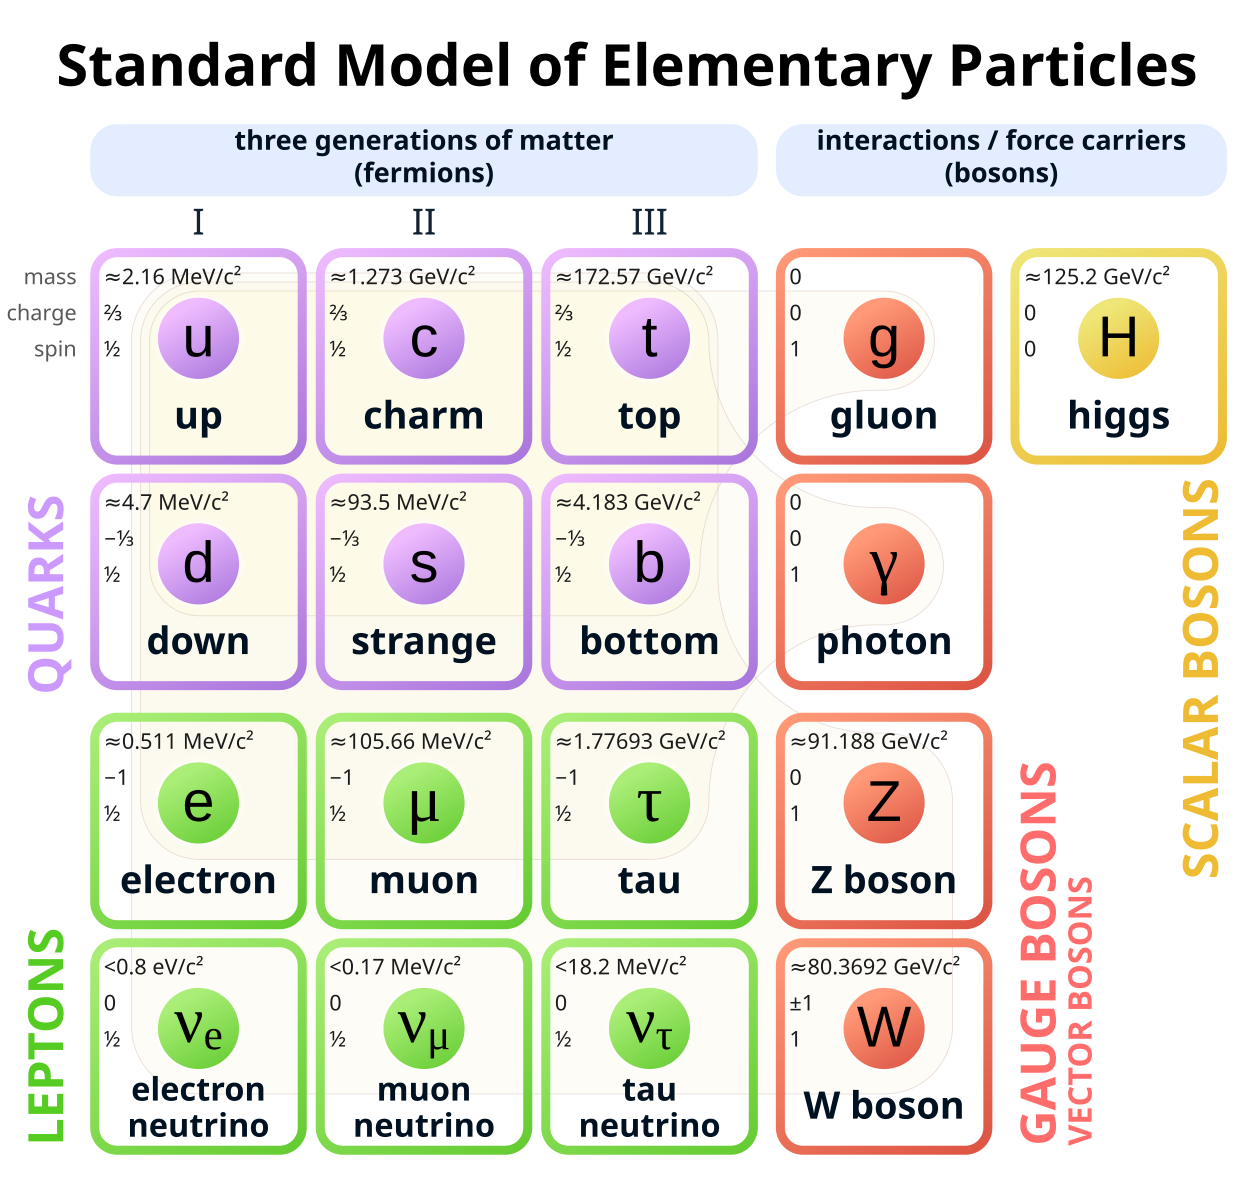
\includegraphics[height=6cm]{images/neutrinos/sm.png}
  \caption{List of the elementary particles in the Standard Model. The antiparticles are not displayed.}
  \label{fig:neutrino:sm}
\end{figure}

Each fermion also possesses an antiparticle of opposite charges and opposite lepton and flavor quantum numbers. Thus, the antiparticle of the electron $e (Q=1, L=1, L_e=1)$, the positron, is defined as $e^+ (Q=-1, L=-1, L_e=-1)$.

The particles of the SM interact with each other via four interactions or forces. Three of these are described by the SM through the exchange of a boson:
\begin{itemize}
  \item The strong force, described by the exchange of a gluon. Only quarks are sensitive to it. This force is very short-range, $\sim 10^{-15}$ m, the size of a nucleus. It's the strong force that allows the cohesion of nuclei inside atoms. As its name indicates, it is the strongest of the four interactions. This interaction has two important properties. It increases with the distance, causing quark confinement: the quarks are never observed individually but uncolored quark combinations, the hadrons, are not affected. It decreases at short distance, creating the asymptotic freedom: the interaction strength become arbitrarily small as the distance between particles decrease.

  \item The electromagnetic force is described by the exchange of a photon. This force has unlimited range, and all the charged particles -- quarks and charged leptons -- are sensitive to it. It is responsible for every electromagnetic effect, like the bonding of electrons to the nucleus. Its relative strength compared to the strong force is 1/137.

  \item The weak force, carried by the $Z^0$ and $W^{\pm}$ bosons. Every fermion is sensitive to it. Its range is $\sim 10^{-18}$ m, about 0.1\% the size of a proton. Its relative strength to the strong force is $10^{-6}$, explaining its name. It is responsible, for instance, of nuclear beta decay many particles decays. We distinguish two types of weak interaction: through neutral currents -- exchange of a $Z^0$ -- and charged currents -- exchange of a $W^{\pm}$ boson.
\end{itemize}

The final force, not described by the Standard Model, is the gravitational force. Its range is infinite and concerns every massive ($m \neq 0$) particle. Its relative strength compared to the strong force is $6\times 10^{-39}$. Extensions to the SM propose a supplementary boson, the graviton, that would be the carrier of the gravitational force, but it has yet to be detected \cite{ParticleDataGroup:2024cfk, carney_graviton_2024}.

\subsection{Interactions and symmetries}

Symmetries are fundamental components of modern particle physics. As described in Noether's theorem \cite{noether_invariant_1971}, the invariance or non-invariance of the physics laws under transformations (translation, rotation, etc.), represented by the formal invariance of the SM Lagrangian ${\cal L}$ under those transformations, implies the conservation of a quantity.
This Lagrangian is the mathematical object that allows us to make quantitative predictions.

The invariance of ${\cal L}$ under translation in space characterizes the conservation of the momentum, while rotational invariance in space leads to the conservation of the angular momentum and invariance under translation in time the conservation of energy, etc. If the transformation is continuous, the sum of the quantum numbers is conserved in an interaction.
Following here again Noether's theorem after having observed that interactions seem to conserve quantities (like the electric charge or the weak isospin), its form is guided by the necessity to be invariant under a local gauge transformation, namely under the $SU(3)_C \bigotimes SU(2)_L \bigotimes U(1)_Y$ gauge group.

Invariance under discrete transformations also conserve quantum numbers. Three discrete transformations are important for the SM:
\begin{itemize}
  \item The parity $P$ symmetry transforms $(\vec{x}, t) \rightarrow (-\vec{x}, t)$, reversing the handedness of space. The momentum therefore becomes $\vec{p} \rightarrow -\vec{p}$ and the helicity $\frac{\vec{p} \cdot \vec{s}}{|\vec{p}|}$, where $\vec{s}$ is the spin, changes sign.

  \item Time reversal $T$ where $(\vec{x}, t) \rightarrow (\vec{x}, -t)$, inverting the initial and final states of an interaction. For example, $A + B \rightarrow C$ becomes $C \rightarrow A + B$. The momentum and the spin both change sign, leaving the helicity unchanged.

  \item Charge conjugation $C$, which replaces the particles by their antiparticles counterpart and vice-versa, leaving the momentum, spin and helicity unchanged.
\end{itemize}

The C, P and their combination CP symmetry were believed to be conserved until 1956, the discovery of their violation \cite{lee_question_1956, wu_experimental_1957, christenson_evidence_1964} in weak interactions revealed the non-triviality of its nature.

The strong and electromagnetic interactions are invariant under all discrete and combined CP transformations. The weak interaction is only invariant under CPT.

The fundamental symmetry CPT -- the combination of C, P and T symmetries --, is an exact symmetry in the SM. This means that any process where the particles are switched with their anti-particles, their helicity is reversed and initial and final state are swapped, must occur with the same probability as the initial process. This implies that the mass, life times, absolute values of electric charge and magnetic moments of particles and antiparticles must be the same. To date, there's no experimental sign of CPT violation.

\subsubsection{Higgs mechanism}

The SM Lagrangian is actually the sum of several parts. The first is the simplest Lagrangian that can be built to respect the Gauge invariance mentioned above and to provide a renormalizable theory. It describes the interaction between fermions and gauge bosons. But alone, this Lagrangian can only describe the interaction of massless particles. This applies in particular to fermions. Indeed, the weak interaction treating differently left-handed and right-handed states, the Lagrangian cannot account for fermion masses via simple terms coupling linearly only right and left-handed fermion fields. Since these fields transform differently under $SU(2)_L$, such terms would break gauge invariance.

Solving this problem requires the spontaneous breaking of the $SU(2)_L \bigotimes U(1)_Y$ gauge symmetry. The second term of the Lagrangian, the Higgs Lagrangian, is introduced by hand for that purpose. The so-called Higgs mechanism introduces the Higgs field, whose non-zero vacuum expectation value breaks the electroweak symmetry, giving masses to the $W$ and $Z$ bosons while keeping the photon massless, and preserving at accessible energies the $U(1)$ gauge symmetry associated with electrodynamics.

Finally, a third Lagrangian term is introduced ad-hoc to account for fermion masses. The Yukawa Lagrangian is designed to couple right-handed and left-handed fermion fields to produce mass terms in a way that preserves gauge invariance and renormalisability. This is achieved via a coupling of the fermions with the Higgs field. After spontaneous symmetry breaking, mass terms appear, proportional to the Higgs field vacuum expectation value and Yukawa couplings, which also describe the coupling of fermions to the Higgs boson. The existence and role of the Higgs field, proposed by Peter Higgs, François Englert, and Robert Brout in 1964 \cite{englert_broken_1964, higgs_broken_1964, higgs_broken_1964-1, guralnik_global_1964}, was experimentally confirmed with the discovery of the Higgs boson by the ATLAS and CMS collaborations at CERN in 2012 \cite{aad_observation_2012, chatrchyan_observation_2012}.

\subsubsection{Flavor Mixing}

Nothing in the fundamental principles governing the weak interaction obliges the fermion mass eigenstates to coincide with the interaction eigenstates. Experimental facts actually push to consider the latter are a superposition of the former. It allows quarks of a given flavor to interact with a flavor of another family (for instance b quarks decaying into c or u quarks), and neutrinos to oscillate by spontaneously change their initial flavor into another one. Flavor mixing in these two sectors are described via the Cabibbo-Kobayashi-Maskawa (CKM) matrix \cite{kobayashi_cp-violation_1973} and Pontecorvo-Maki-Nakagawa-Sakata matrix \cite{maki_remarks_1962} matrices, respectively.

In the case of neutrinos, This topic will be addressed in further details in Section \ref{sec:th:osc}. With 3 generations of particles, these 3*3 matrices have to contain complex terms via which the SM accounts for CP violation.

% Decrire le model standard -> Regarder theses LHC / Olga Kochebina

\subsection{Limits of the standard model}

The SM has been successful at describing many of phenomena observed in experiments. However, some questions remain unanswered, among which:

\begin{itemize}
  \item Dark matter and dark energy. Cosmological observations -- such as the acceleration of the expansion of the universe and the rotational speed of galaxies, for example -- indicate the presence of unknown energy and matter in the universe. The $\Lambda$CDM model \cite{bull_beyond_2016, perivolaropoulos_challenges_2022} indicates that only 4.5\% of the total energy in the universe is described by the SM. The supplementary mass -- dark matter -- accounts for 22.5\% of the missing energy and the rest is dark energy.
  \item Baryon Asymmetry of the universe. The universe is mainly made of matter. The Sakharov theory \cite{sakharov_violation_1991} to explain the deficit of antimatter require the breaking of the C and CP symmetries. The CP violation is allowed in the strong sector, but not to the magnitude necessary to explain the quasi absence of baryon anti-matter. Other mechanism must exist to explain this deficit.
  \item Fermion masses. The large mass difference between the fermions is not explained by the SM.
  \item The SM includes 26 numerical parameters, the values of which are determined only through experimental measurements. At least 20 of these parameters are related to flavor physics. In electroweak theory nothing dictates the values of the interaction couplings and masses. This reflects a deeper limitation of the model, as it provides no theoretical explanation for the values of these parameters, which suggests that a more fundamental theory may be required.
  \item Strong CP problem. Theoretically it is possible to have violation of CP symmetry in strong interactions. Experimentally, however, no such asymmetry has been found, implying that the coefficient of this term is very close to zero. This fine-tuning is considered unnatural.
  \item Non-unification of couplings. The gauge couplings of the SU(3), SU(2) and U(1) groups are independent quantities. Due to higher-order corrections, each of these is actually a function of the typical energy scale $Q$ relevant to the process. In many grand unified theories the three gauge couplings are predicted to meet at some high energy unification. However, this unification does not occur when the couplings are extrapolated using the SM model expression.
  \item Gravitation. The SM do not include the Gravitational interaction and is incompatible with the general relativity.
\end{itemize}


% \marginpar{Limite du model standard - Interessant/justifier etudier les neutrinos -> violation de CP ? Pb des masses ?}
\section{The Neutrinos}
\label{sec:neutrino:th}

As introduced in the previous section, the neutrino are the neutral leptons of the Standard Model (SM). They were first theorized by Wolfgang Ernst Pauli in 1978 \cite{pauli_dear_1978} to solve the problem of the $\beta$-decay continuous spectrum. Indeed, if the $\beta$-decay was a two body reaction $^A_Z X \rightarrow ^A_{Z + 1}Y + e^{-}$, the conservation of momentum would force the charged lepton to be mono-energetic, but the measured spectrum was continuous. To solve this problem Pauli theorized the emission of a neutral particle $^A_Z X \rightarrow ^A_{Z + 1}Y + e^{\pm} + \nu$, the neutrino. This particle had to be light, neutral, and interact weakly with matter.

We must wait 1956 for a collaboration led by Frederick Reines and Clyde Cowan for the first observation of the neutrino \cite{reines_neutrino_1956, cowan_detection_1956} via the Inverse Beta Decay (IBD) reaction
\begin{equation}
  \bar{\nu} + p \rightarrow e^+ + n
\end{equation}

Following this discovery, numerous experiments were set up to study its properties. Some notable discoveries include the discovery in 1962, by a collaboration led by Leon Lederman, Melvin Schwartz and Jack Steinberger, of the muon neutrino flavor \cite{danby_observation_1962}.

Soon after, the Homestake experiment, which was measuring the neutrino produced by the proton-proton fusion cycle in the sun, reported a deficit of factor $\sim 3$ \cite{davis_review_1994} in comparison to the Standard Solar Model predictions. This anomaly, referred as the \textit{solar neutrino problem} remained unexplained until the neutrino oscillation was theorized and proven. Bruno Pontecorvo first suggested a $\nu \leftrightarrow \bar{\nu}$ oscillation \cite{pontecorvo_mesonium_1957}, later revisited by Maki et al.\ to a two flavor oscillation $\nu_e \leftrightarrow \nu_\mu$ \cite{maki_remarks_1962}. The discovery of the $\tau$ lepton 1976 \cite{perl_evidence_1975} and its associated neutrino $\nu_\tau$ \cite{kodama_observation_2001} led to the extension to three flavor oscillation.

This three flavor oscillation was confirmed by the observation of the $\nu_\mu \leftrightarrow \nu_\tau$ oscillation \cite{fukuda_evidence_1998} in 1998 by the Super-Kamiokande experiment.

\subsection{Coupling and interactions}

The SM, as originally defined, contains no right-handed neutrino (right helicity) since only left-handed neutrinos have been observed \cite{goldhaber_helicity_1958}, implying that the neutrinos are massless. Neutrinos actually do have a very small mass, with the current best limit $m_\nu < 0.45$ eV at 90\% confidence level, obtained from the measurement of the electron energy spectrum in tritium beta decay by the KATRIN experiment \cite{aker_direct_2024}. They only couple -- interact -- through the $W^{\pm}$ and $Z^0$ bosons. The coupling with a $W^{\pm}$ boson is the \textit{charged current}, a charge is exchanged via the $W$ boson, and coupling with $Z^0$ is the neutral current, no charge is exchanged. The Feynman diagrams representing those interactions are presented in Figure \ref{fig:neutrinos:currents}.

\begin{figure}
  \centering
  \begin{subfigure}[t]{0.48\linewidth}
    \centering
    \feynmandiagram[horizontal=a to b] {
      a -- [boson, edge label=\(W^{\pm}\)] b,
      f1 [particle=\(\nu_l\)] -- [fermion] b -- [fermion] f2 [particle=\(l\)]
    };
  \end{subfigure}
  \hfill
  \begin{subfigure}[t]{0.48\linewidth}
    \centering
    \feynmandiagram[horizontal=a to b] {
      a -- [boson, edge label=\(Z^0\)] b,
      f1 [particle=\(\nu\)] -- [fermion] b -- [fermion] f2 [particle=\(\nu\)]
    };
  \end{subfigure}
  \caption{Feynman diagrams of the charged current (\textbf{on the left}) and the neutral current (\textbf{on the right}) for a lepton $l$ and it corresponding neutrino $\nu_l$.}
  \label{fig:neutrinos:currents}
\end{figure}

As explained in Section \ref{sec:neutrinos:sm}, those interactions preserve the lepton quantum number $L$. In the absence of neutrino mass, the lepton flavor numbers $L_e$, $L_\mu$ and $L_\tau$ are also exactly conserved. However, the existence of neutrino masses allow for lepton flavor violating transition such as the oscillation $\nu_\alpha \rightarrow \nu_{\beta \neq \alpha}$ but also process such as $\mu^+ \rightarrow e^+ + \gamma$ or $\mu^+ \rightarrow e^+ e^+ e^-$. The latter that are heavily suppressed -- their probability of occurring is extremely low in comparison to other processes -- in the absence of new physics \cite{glashow_weak_1970}.


%\subsubsection{First theories}

%\subsubsection{Discovery}

%\subsubsection{Milestones and anomalies}

\subsection{Oscillation}
\label{sec:th:osc}

Neutrino oscillations occur due to the fact that the flavor states, in which neutrinos are produced and detected, are quantum superposition of mass eigenstates. This results in neutrinos changing their flavor as they propagate, with the oscillation parameters depending on the differences in the squared masses of the mass eigenstates. More strictly speaking, their mass induces a mismatch between the \textit{flavor states} $\ket{\nu_e}$, $\ket{\nu_\mu}$ and $\ket{\nu_\tau}$ which are the state in which the particle interacts -- the states in the diagrams in Figure \ref{fig:neutrinos:currents} -- and the \textit{mass states} $\ket{\nu_1}$, $\ket{\nu_2}$ and $\ket{\nu_3}$ which hold the momentum and mass of the particle.

Thus, the flavor state $\ket{\nu_\alpha}$ is a quantum superposition of mass eigenstates, and can be written
\begin{equation}
  \ket{\nu_\alpha} = \sum_{i=1}^3 U_{\alpha, i} \ket{\nu_i}
\end{equation}
and reciprocally
\begin{equation}
  \ket{\nu_i} = \sum_{\alpha \in e,\mu,\tau} U^*_{\alpha, i} \ket{\nu_\alpha}
\end{equation}
where $i$ indexes the mass states, $\alpha$ the flavor states and the $U_{\alpha, i}$ are the mixing elements that govern the probability amplitudes for the neutrino flavor transitions. In the three-families framework, this mixing is represented by the $3 \times 3$ Pontecorvo-Maki-Nakagawa-Sakata matrix \cite{maki_remarks_1962} $U_{\text{PMNS}}$
\begin{equation}
  \begin{pmatrix}
    \ket{\nu_e} \\
    \ket{\nu_\mu} \\
    \ket{\nu_\tau}
  \end{pmatrix} = U_{\text{PMNS}} \begin{pmatrix}
    \ket{\nu_1} \\
    \ket{\nu_2} \\
    \ket{\nu_3}
  \end{pmatrix} = \begin{pmatrix}
  U_{e1} & U_{e2} & U_{e3} \\
  U_{\mu 1} & U_{\mu 2} & U_{\mu 3} \\
  U_{\tau 1} & U_{\tau 2} & U_{\tau 3}
  \end{pmatrix} \begin{pmatrix}
    \ket{\nu_1} \\
    \ket{\nu_2} \\
    \ket{\nu_3}
  \end{pmatrix}
\end{equation}
This matrix is considered to be unitary, but this property still needs to be corroborated \cite{parke_unitarity_2016}. Now, considering a neutrino produced as $\ket{\nu_\alpha}$ that propagates over a distance $x$ during a time $t$, the Schrödinger equation \cite{schrodinger_undulatory_1926} can be written as:
\begin{equation}
  \label{eq:neutrino:schro}
  \ket{\nu_\alpha(x, t)} = \sum_{i=1}^3 U_{\alpha, i} e^{-i(E_it-p_ix)} \ket{\nu_i}
\end{equation}
where $E_i$ and $p_i$ stand for the energy and momentum of the neutrino mass states respectively. By going back from the mass space to the flavor space, Eq. \ref{eq:neutrino:schro} becomes:
\begin{equation}
  \ket{\nu_\alpha(x, t)} = \sum_{\beta \in e,\mu,\tau} U^*_{\beta, i} \left( \sum_{i=1}^3 U_{\alpha, i} e^{-i(E_it-p_ix)} \right) \ket{\nu_\beta}
\end{equation}

A neutrino created as $\nu_\alpha$ thus propagates as the linear superposition of the three flavor states. Because the mass of the neutrino is extremely small, we can consider that they are ultra-relativistic ($E \sim p >> m$). Using natural units $(c = \hbar = 1)$:
\begin{equation}
  \label{eq:neutrino:e_eq_p}
  E_i = \sqrt{p^2 + m_i^2} \simeq p + \frac{m_i^2}{2p} \simeq E + \frac{m_i^2}{2E}
\end{equation}
then the probability to observe a neutrino produced in state $\ket{\nu_\alpha}$ in a state $\ket{\nu_\beta}$ can be written \footnote{Actually Eq. \ref{eq:neutrino:e_eq_p} and \ref{eq:neutrino:prob} make a few more assumptions, such as the fact that every mass state has the same momentum. ``Paradoxes of Neutrino Oscillations'' from Akhmedov and Smirnov \cite{akhmedov_paradoxes_2009} go through them and demonstrate the validity of the method presented in this chapter.}:
\begin{equation}
  \label{eq:neutrino:prob}
  P_{\nu_\alpha \rightarrow \nu_\beta} = | \braket{\nu_\beta}{\nu_\alpha} |^2 = \sum_{i,j=1}^3 U^*_{\alpha,i} U_{\beta,i} U^*_{\alpha, j} U_{\beta, j} e^{-i \frac{\Delta m^2_{ji} L}{2E}}
\end{equation}
where $L = ct$ is the propagation distance of the neutrino, $E$ is the neutrino energy and $\Delta m^2_{ji} = m^2_j - m^2_i$ is the \textit{mass splitting}, the difference between the square of the eigenvalues of two mass states.

Under unitary assumptions, the PMNS matrix can also be decomposed in three rotational matrices:
\begin{equation}
  U_{\text{PMNS}} = \begin{pmatrix}
    1 & 0 & 0 \\
    0 & \cos \theta_{23} & \sin \theta_{23} \\
    0 & -\sin \theta_{23} & \cos \theta_{23} \\
  \end{pmatrix} \begin{pmatrix}
    \cos \theta_{13} & 0 & \sin \theta_{13} e^{-i\delta_{\text{CP}}}\\
    0 & 1 & 0 \\
    -\sin \theta_{13} e^{i\delta_{\text{CP}}} & 0 &  \cos \theta_{13} \\
  \end{pmatrix} \begin{pmatrix}
    \cos \theta_{12} & \sin \theta_{12} & 0 \\
    -\sin \theta_{12} & \cos \theta_{12} & 0 \\
    0 & 0 & 1 \\
  \end{pmatrix}
\end{equation}
where the parameters $\theta_{12}$, $\theta_{23}$, $\theta_{13}$ are the \textit{mixing angles}. The parameter $\delta_{\text{CP}}$ is a CP violation phase that quantifies the matter-antimatter asymmetry in the lepton sector. The parameters $\theta_{12}$ and $\Delta m^2_{21}$ are commonly attributed to a so-called \textit{solar sector}, while the parameters $\theta_{13}$ and $\Delta m^2_{31}$ belong to the \textit{reactor sector} and $\theta_{23}$ and $\Delta m^2_{32}$ the \textit{atmospheric sector}. The neutrino oscillation is thus characterized by 7 parameters: the three mixing angles $(\theta_{12}, \theta_{13}, \theta_{23})$, the three mass splitting $(\Delta m^2_{21}, \Delta m^2_{31}, \Delta m^2_{32})$ and the CP violation phase $\delta$.
These three mass splittings are constrained by the relation
\begin{equation}
  \Delta m^2_{21} + \Delta m^2_{32} - \Delta m^2_{31} = 0
\end{equation}

The neutrinos interact weakly with matter. But even so, the travel through dense matter, such as the Earth's crust, can impact their propagation probability. These \textit{matter effects} where introduced by Lincoln Wolfenstein, Stanislas Mikheyev and Alexei Smirnov in 1978 \cite{wolfenstein_neutrino_1978}. They result from forward elastics scattering of neutrinos with the medium (the momentum of the neutrino is unchanged). The charged and neutral current Feynman diagrams are presented in Figure \ref{fig:neutrinos:msw}. This results in a supplementary potential in the Hamiltonian, impacting the oscillation probability.


\begin{figure}[ht]
  \centering
  \begin{subfigure}[t]{0.48\linewidth}
    \centering
    \feynmandiagram[vertical=a to b] {
      f1 [particle=\(\nu_e\)] -- [fermion] a -- [fermion] o1 [particle=\(e^{-}\)],
      a -- [boson, edge label=\(W^{-}\)] b,
      f2 [particle=\(\nu_e\)] -- [anti fermion] b -- [anti fermion] o2 [particle=\(e^{-}\)]
    };
  \end{subfigure}
  \begin{subfigure}[t]{0.48\linewidth}
    \centering
    \feynmandiagram[vertical=a to b] {
      f1 [particle=\(\nu_{e, \mu, \tau}\)] -- [fermion] a -- [fermion] o1 [particle=\(\nu_{e, \mu, \tau}\)],
      a -- [boson, edge label=\(Z^{0}\)] b,
      f2 [particle={$e^{-},p,n$}] -- [anti fermion] b -- [anti fermion] o2 [particle={$e^{-},p,n$}]
    };
  \end{subfigure}
  \caption{Feynman diagrams of the of charged current matter effect (\textbf{on the left}) and the neutral current matter effect (\textbf{on the right}). Only the electronic neutrino is sensitive to charged current, whereas every neutrinos are sensitive to neutral current.}
  \label{fig:neutrinos:msw}
\end{figure}

\subsection{Phenomenology}
\label{sec:neutrino:pheno}

The neutrinos experiments can be divided into two main categories: the disappearance experiments, which observe a deficit of a specific flavor of neutrinos in the detector compared with the expected source flux, and the appearance experiments that search for an excess of a flavor. By placing them at different distances -- baselines -- we can favor the appearance or disappearance of different neutrino flavors. As an illustration of the effect of the baseline, the survival probability of $\bnue$ with respect to the baseline is presented in Figure \ref{fig:neutrino:baseline_effect}.

\begin{figure}[ht]
  \centering
  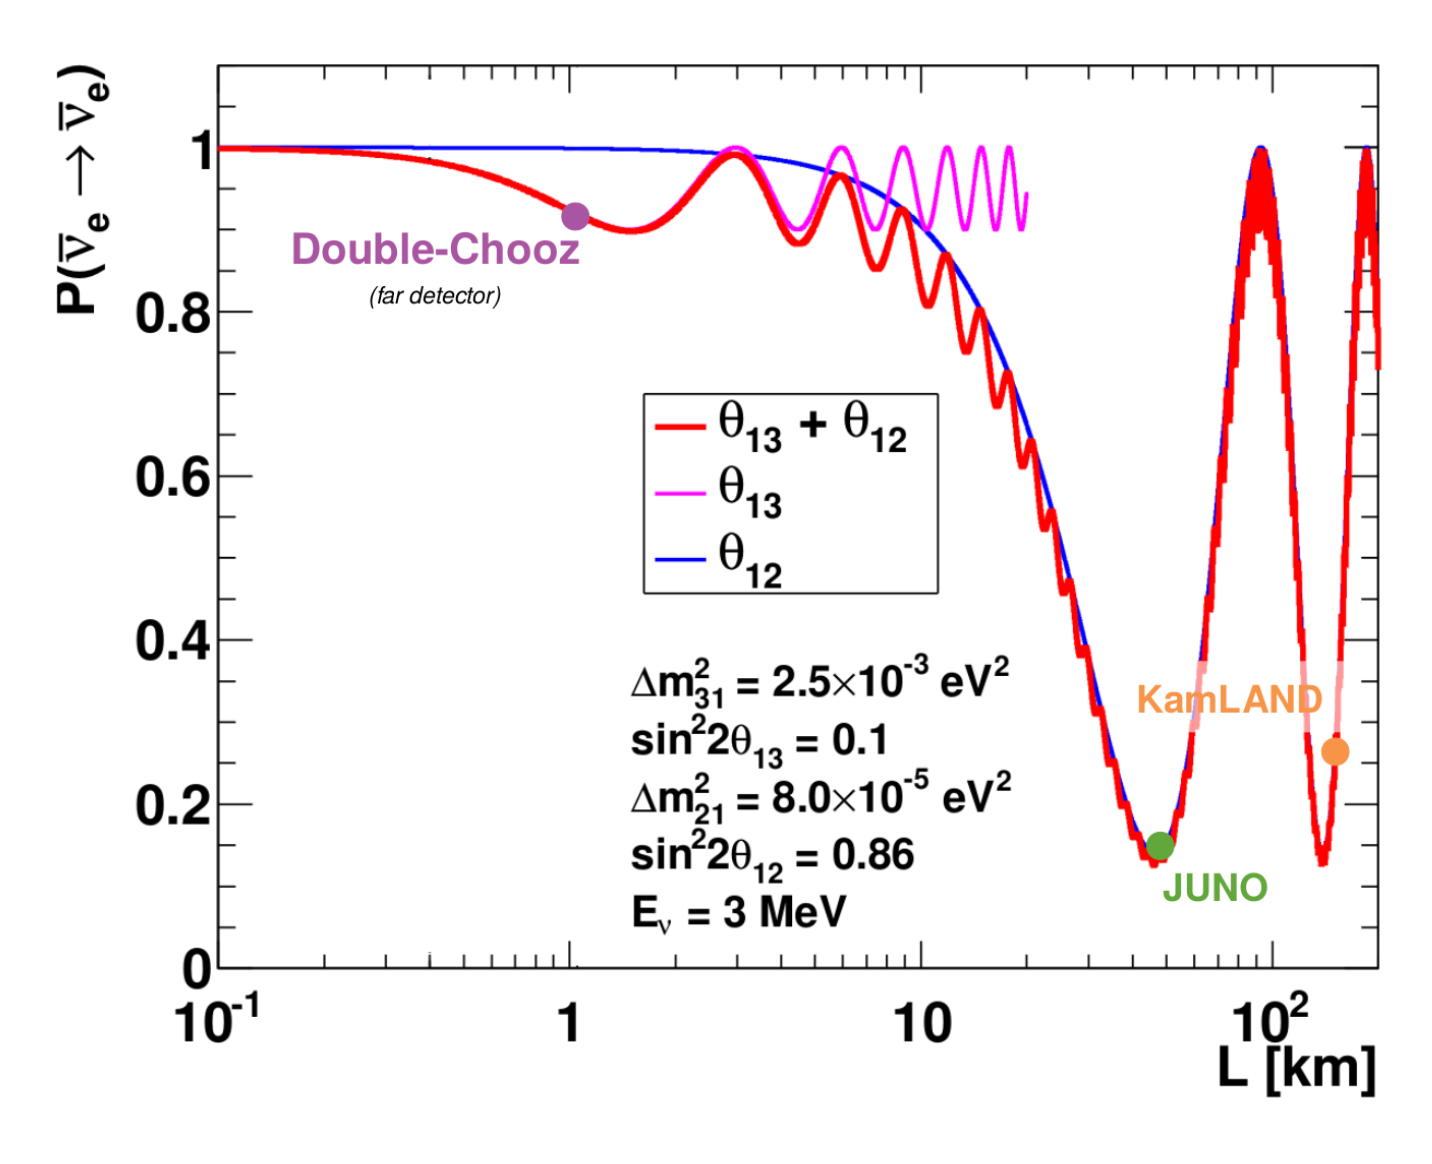
\includegraphics[height=7cm]{images/neutrinos/baseline_effect.png}
  \caption{Survival probability of $\bar{\nu}_e$ as a function of the baseline. The energy of the neutrinos is 3 MeV. The baseline of Double-Chooz, JUNO and KamLAND are reported. Figure taken from Ref. \cite{lebrin_towards_2022}.}
  \label{fig:neutrino:baseline_effect}
\end{figure}

The experiments are also characterized by the neutrino sources they observe. For neutrino studies, the common sources are solar neutrinos, atmospheric neutrino produced from the interactions of high energy particles in the upper atmosphere, accelerators by firing particle beams on a target, and nuclear power plant reactors.

One of the major questions right now is the Mass Ordering (MO), the sign of the mass splitting terms $\Delta m^2_{31}$, and thus $\Delta m^2_{32}$, is not known. We consider two hypotheses: Normal Ordering (NO) where $m_1 < m_2 < m_3$ and the Inverted Ordering (IO) where $m_3 < m_1 < m_2$. An illustration of the MO is presented in Figure \ref{fig:neutrino:nmo}. This topic will be further discussed in Section \ref{sec:neutrino:questions}.

\begin{figure}
  \centering
  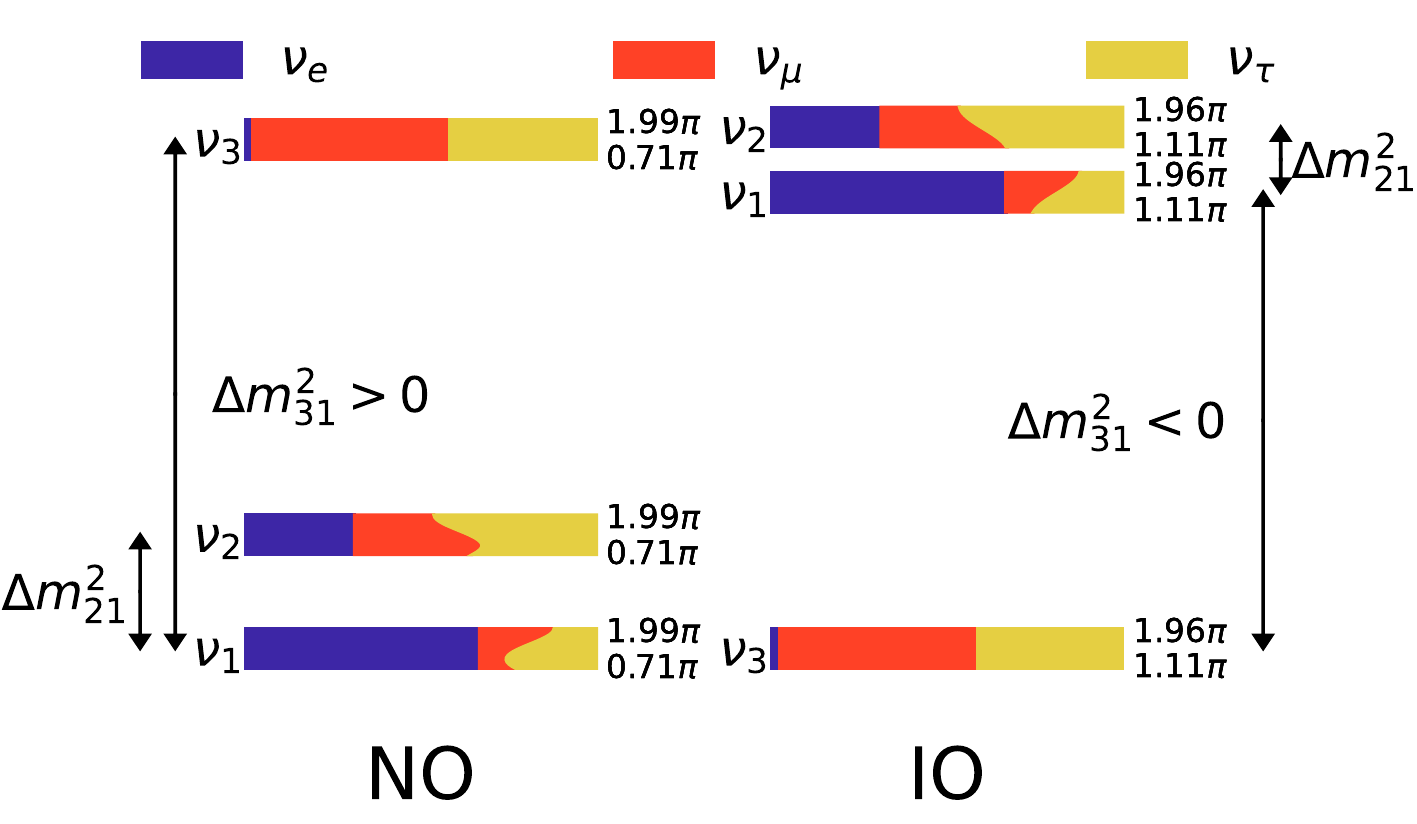
\includegraphics[height=7cm]{images/neutrinos/nmo.png}
  \caption{Illustration of the Mass Ordering, on the left the Normal Ordering and on the right the Inverted Ordering.}
  \label{fig:neutrino:nmo}
\end{figure}

\subsubsection{Solar sector ($\theta_{12}$, $\Delta m^2_{21}$)}

The measurement of the solar sector parameters $\theta_{12}$ and $\Delta m^2_{21}$ has been done in two different ways. From the measurements of the solar neutrino flux in experiments like Super Kamiokande \cite{super-kamiokande_collaboration_solar_2016} and by extracting the parameter from the reactor $\bnue$ spectrum, as done by the KamLand-Zen experiment \cite{suzuki_results_2005, kamland_collaboration_reactor_2013}. Those results are further constrained by measurements of short-baseline experiments and accelerator data. The Particle Data Group (PDG) in its latest edition \cite{ParticleDataGroup:2024cfk} reports the value from global fit efforts from \cite{super-kamiokande_collaboration_solar_2016, kamland_collaboration_reactor_2013}

\begin{equation*}
  \sin^2\theta_{12} = 0.307^{+0.013}_{-0.012}
\end{equation*}
\begin{equation*}
  \Delta m^2_{21} = 7.53 \pm 0.18 \cdot 10^{-5} \text{ eV}^2
\end{equation*}

The intervals are 68\% confidence level. The CPT invariance is assumed.

\subsubsection{Reactor sector ($\theta_{13}$)}

Direct measurements of $\theta_{13}$ are currently derived from the reactor $\bnue$ disappearance at short baseline $L \sim 1$ km. Alternatively, limits can also be obtained from solar neutrino data or accelerator based $\nu_\mu \rightarrow \nu_e$ experiments. The PDG reports its best value as the average of the results T2K \cite{abe_measurements_2023}, DayaBay \cite{daya_bay_collaboration_precision_2023, daya_bay_collaboration_new_2016}, Double-Chooz \cite{de_kerret_double_2020} and Reno \cite{shin_observation_2020, reno_collaboration_measurement_2018}

\begin{equation*}
  \sin^2\theta_{13} = 2.19 \pm 0.07
\end{equation*}


The intervals are 68\% confidence level. The CPT invariance is assumed.

\subsubsection{Atmospheric sector ($\theta_{23}$, $\Delta m^2_{32}$) and $\delta_{\text{CP}}$)}

The parameters $\theta_{23}$ and $\Delta m^2_{32}$ are currently constrained by the measurements the relative fluxes of atmospheric neutrino flavors and by accelerator-based experiments. The mass splitting term can also be extracted from the $\bnue$ spectrum at short baselines. The PDG uses the results of IceCube \cite{icecube_collaboration_measurement_2023}, T2K \cite{abe_measurements_2023}, NOvA \cite{the_nova_collaboration_improved_2022}, MINOS \cite{minos_collaboration_precision_2020} and Super Kamiokande (SK) \cite{super-kamiokande_collaboration_atmospheric_2018} for $\theta_{13}$. For $\Delta m^2_{31}$, they also use the data from Daya Bay \cite{daya_bay_collaboration_precision_2023} and RENO \cite{reno_collaboration_measurement_2018}.

\textbf{Assuming normal ordering}

\begin{equation*}
  \sin^2\theta_{23} = 0.553^{+0.016}_{-0.024}
\end{equation*}
\begin{equation*}
  \Delta m^2_{32} = 2.445 \pm 0.028 \cdot 10^{-3} \text{ eV}^2
\end{equation*}

\textbf{Assuming inverted ordering}
\begin{equation*}
  \sin^2\theta_{23} = 0.558^{+0.015}_{-0.021}
\end{equation*}
\begin{equation*}
  \Delta m^2_{32} = -2.529 \pm 0.029 \cdot 10^{-3} \text{ eV}^2
\end{equation*}

The CP violation phase $\delta_{\text{CP}}$ is measured from the $\nu_e$ appearance in atmospheric and accelerator experiments. PDG uses the data from T2K \cite{abe_measurements_2023}, NOVA \cite{the_nova_collaboration_improved_2022} and Super Kamiokande \cite{super-kamiokande_collaboration_atmospheric_2018}. The reported value is in $\pi$ radians with $0 < \delta_{\text{CP}} < 2 \pi$. This value of $\delta_{\text{CP}}$ assumes Normal Ordering.

\begin{equation*}
  \delta_{\text{CP}} = 1.19 \pm 0.22
\end{equation*}

The intervals are 68\% confidence level. The CPT invariance is assumed.

\subsection{Open questions}
\label{sec:neutrino:questions}

Neutrino experiments have continued to produce more and more precise and refined results over the last 25 years. However, some questions remain unanswered and will be at the center of attention of the neutrino physics community for the years to come. Some of them are reviewed in this section.

% Majorana vs dirac
%
% absolute neutrino mass scale
%
% Mass ordering
%
% \theta_{23} octant
%
% CP symmetrie
%
% sterile

\subsubsection{Nature of the neutrino}

The particles in the SM are Dirac particles (i.e.\ there is a distinction between particles and antiparticles). The modern model of neutrino interaction and oscillation has been developed under this postulate. However, Ettore Majorana in 1937 formulated another way to introduce mass terms in the SM Lagrangian \cite{majorana_teoria_1937}. The condition for this mass term is only applicable to the neutrino. If the neutrino is a Majorana particle, meaning it is its own antiparticle, lepton number violation would occur during certain processes such as neutrinoless double beta decay. This violation is predicted because in Majorana interactions, neutrinos can annihilate themselves, violating lepton number conservation by two units. To determine the nature of the neutrino (Majorana or Dirac nature), physicist observe the rare phenomenon of $\beta\beta$ decay -- double beta decay:
\begin{equation}
  ^{A}_{Z}X \rightarrow ^{A}_{Z+2}Y + e^- + e^- + \bnue + \bnue
\end{equation}
In this scenario, if the neutrino are Majorana particles, one could observe a theoretically rarer event $0\nu\beta\beta$ decay:
\begin{equation}
  ^{A}_{Z}X \rightarrow ^{A}_{Z+2}Y + e^- + e^-
\end{equation}
where the two neutrinos annihilate in the interaction. The signature would be the presence of quasi mono-energetic events at the higher end of the $\beta\beta$ decay energy spectrum.

The implication of the Majorana nature of the neutrino implies, among others:
\begin{itemize}
  \item The lepton number violation.

  \item Possible explanation of small neutrino masses via seesaw mechanism \cite{yanagida_horizontal_1980}.

  \item Open the possibility of generating the baryon asymmetry via leptogenesis.
\end{itemize}

As of today, the nature of the neutrino hasn't been established.

\subsubsection{Absolute mass of the neutrino}

Studies of neutrino oscillation allow us to measure the mass splitting terms $\Delta m^2_{ij} = m^2_{i} - m^2_{j}$ but do not provide information about the absolute mass scale of the neutrinos.
The most stringent upper limits on the absolute neutrino mass come from the KATRIN experiment, which measures the electron energy spectrum in tritium beta decay. By precisely studying the tail of this spectrum, where small energy differences due to the neutrino mass can manifest, KATRIN is able to constrain the neutrino mass with a high degree of sensitivity. The latest result gives an upper limit at a 90\% confidence level of $m_\nu < 0.45$ eV \cite{aker_direct_2024}.

\subsubsection{Neutrino Mass Ordering (NMO)}

As introduced in Section \ref{sec:neutrino:pheno}, current experiments are only sensitive to $|\Delta m^2_{32}|$, blinded to the sign of the mass split. We are thus unable to differentiate between the Normal Ordering (NO) $m_1 < m_2 < m_3$ and the Inverted Ordering (IO) $m_3 < m_1 < m_2$. The nature of the NMO has important implications:
\begin{itemize}
  \item It will help in the determination of the lower limit of the mass scale.
  \item The nature of the neutrino mass ordering has significant implications for various experiments, particularly neutrinoless double beta decay ($0\nu\beta\beta$). If the mass ordering is inverted, the effective mass for $0\nu\beta\beta$ is likely to be higher, which would increase the decay's detectability. Conversely, a normal ordering would imply a lower effective mass, making detection more challenging.
  \item The current $\delta_{\text{CP}}$ measurements have different minima depending on the mass ordering as illustrated in Figure \ref{fig:neutrino:chi2_proj}.
  \item More broadly, knowledge of the mass ordering and the neutrino mass scale have impacts on the generation of lepton in early universe and cosmology \cite{hannestad_cosmology_2016}.
\end{itemize}

\begin{figure}[ht]
  \centering
  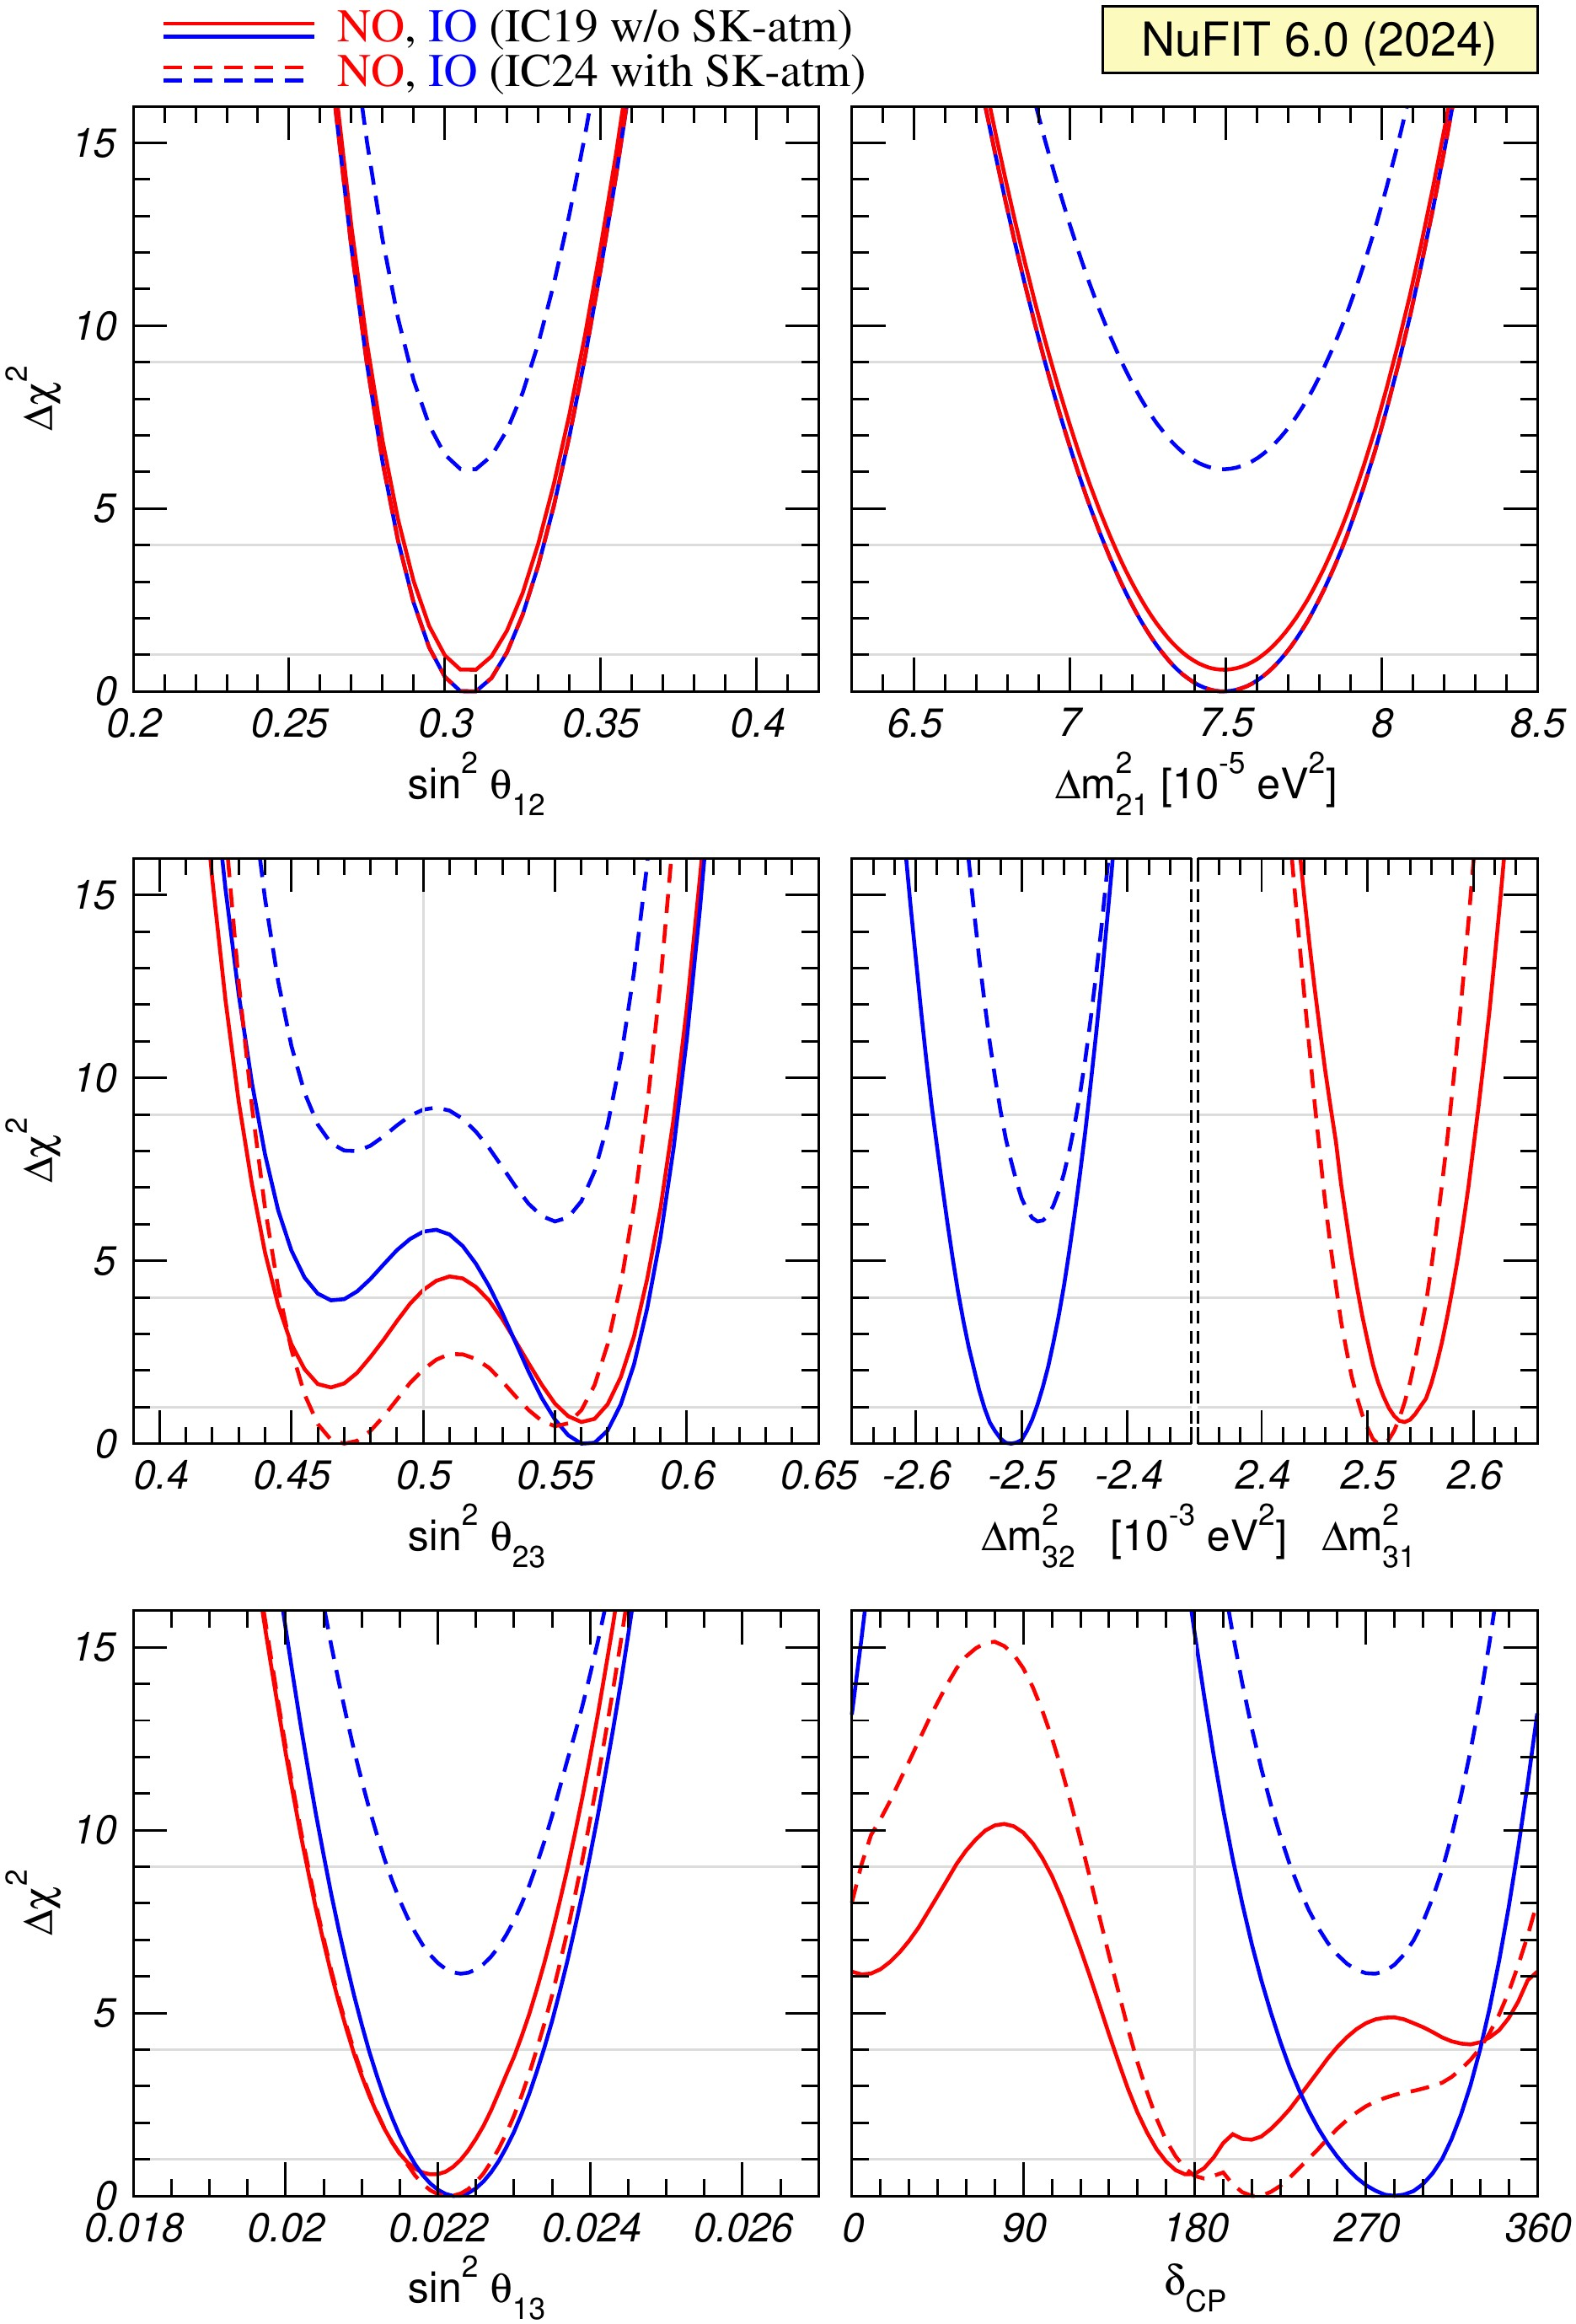
\includegraphics[width=8cm]{images/neutrinos/chi2_proj.jpg}
  \caption{Global 3$\nu$ oscillation analysis. The red (blue) curves are for Normal (Inverted) Ordering. The solid (dashed) lines are obtained without (with) the inclusion of the tabulated atmospheric $\chi^2$ data from SK and IC. As atmospheric mass-squared splitting we use $\Delta m^2_{31}$ for NO and $\Delta m^2_{32}$for IO. Analysis and plots from the NuFit analysis group \cite{esteban_nufit-60_2024, noauthor_nufit_nodate}.}
  \label{fig:neutrino:chi2_proj}
\end{figure}

The determination of the mass ordering will probably be solved in the next decade. Multiple experiments under construction have this topic as part of their main physics program, notably the Jiangmen Underground Neutrino Observatory (JUNO) \cite{juno_collaboration_juno_2022} -- the subject of this thesis -- via the measurement of the $\bnue$ spectrum from nuclear reactors; the long-baseline DUNE experiment \cite{abi_long-baseline_2020} which will detect neutrinos from the Fermilab accelerator; KM3Net/ORCA and Hyper-Kamiokande through the measurements of the atmospheric neutrino flux \cite{aiello_determining_2021, abe_hyper-kamiokande_2018}.

\subsubsection{Octant of $\theta_{23}$}

The latest results from the NuFit analysis group \cite{esteban_nufit-60_2024} show two minima for $\theta_{13}$ (Fig. \ref{fig:neutrino:chi2_proj}), one in the lower octant $\theta_{23} < \pi/4$ and one in the upper octant $\theta_{23} > \pi/4$. This octant has implications for the oscillation and neutrino mass theories. It will be measured by future neutrino experiments such as DUNE and HK.

\subsubsection{Breaking of CP symmetry in the lepton sector}

The CP symmetry is known to be broken in the baryon sector \cite{christenson_evidence_1964} however its violation in the lepton sector is still unknown. The CP violation exists if the PMNS matrix possesses an imaginary part, i.e.\ if $\text{Im}(e^{i\delta_{CP}}) \neq 0$. The latest measurements (Fig. \ref{fig:neutrino:chi2_proj}) do not give any certainties about the value of $\delta_{CP}$; it will be determined by future experiments such as DUNE and HK. The violation of CP in the leptonic sector has strong implications for the matter-antimatter asymmetry in the universe.

\subsubsection{Sterile neutrino}

Sterile neutrinos are hypothetical particles that extend the Standard Model by introducing a fourth, non-interacting neutrino family. They have been proposed to explain certain anomalies observed in short-baseline neutrino experiments, such as the LSND \cite{lsnd_collaboration_evidence_2001} and MiniBooNE \cite{miniboone_collaboration_significant_2018} experiments, where observed oscillations cannot be accounted for by the known three neutrino flavors.
This sterile neutrino would not interact with the other particles of the SM except via gravity and could be observed only via the oscillations of $\nu_e,\nu_\mu,\nu_\tau \rightarrow \nu_s$ where $\nu_s$ would be this hypothetical fourth sterile family. This theory has been proposed multiple times to explain anomalies in the oscillation's data, but for now no studies have concluded on the existence of the sterile neutrino. One of the possible probes for this fourth family would be the measurement of the non-unitarity of the PMNS matrix, meaning that $\nu_e$ is a linear combination of $\nu_1, \nu_2, \nu_2$ and a theoretical $\nu_4$. This unitarity test can be done via precise measurements of the mixing angles.
\end{document}
